\documentclass[11pt]{beamer}
\usepackage{pifont}
\usepackage[english]{babel}
\usepackage[backend=biber,style=authoryear-comp,sorting=none]{biblatex}
\usepackage{graphicx}
\usepackage{caption}
\usepackage{subcaption}
\usepackage{csquotes}
\usepackage{picture}
\usepackage{tabularx}
\usepackage{booktabs}

\addbibresource{biblio.bib}
\captionsetup[table]{singlelinecheck=false, justification=raggedright, labelfont=normalfont}
\newcolumntype{C}{>{\centering\arraybackslash}X}

\definecolor{kyushu}{RGB}{133, 2, 62}
\setbeamercovered{transparent}
\setbeamertemplate{itemize items}{\ding{108}}
\setbeamercolor{itemize item}{fg=kyushu}
\setbeamertemplate{itemize subitem}{--}
\setbeamercolor{itemize subitem}{fg=black}

\setbeamerfont{frametitle}{series=\bfseries}
\captionsetup{font=tiny}
\setbeamertemplate{footline}[frame number]
\setbeamerfont{footnote}{size=\tiny}

\setbeamercolor{frametitle}{bg=kyushu, fg=white}
\setbeamercolor{title}{bg=kyushu, fg=white}

\title{\textbf{Importance of N$_2$H$_x$ Reaction Pathways to Optimize Okafor Reduced Mechanism for NH$_3$/H$_2$ Flame Chemistry}}
\subtitle{}
\institute{Department of Mechanical Engineering\\Reactive Gas Dynamics Laboratory}
\author{UROTHIYIL Aahil Ashraf (1TE23533T)}

\begin{document}

\frame{
    \titlepage
}

\begin{frame}
	\frametitle{Research Background}
	Traditional sources of energy rely on combustion of fossil fuels that produce carbon emissions which have adverse effects on the environment:
	\begin{itemize}
		\item Global Warming
		\item Climate Change
	\end{itemize}
	New carbon-free alternative fuels are needed to prevent exacerbating the effects of carbon pollutants
	\begin{itemize}
		\item The Japanese government seeks to reduce total greenhouse gas emissions by 46\% before 2030
		\item By 2050, Japan envisions its cities to be carbon-neutral
	\end{itemize}
\end{frame}

\begin{frame}
	\frametitle{Research Background}
	Ammonia, NH$_3$, is gaining interest among researchers for its potential to meet energy needs in a variety of applications.\\\vspace{10pt}
	Ammonia is a suitable fuel for combustion application because:
	\begin{columns}
		\begin{column}{0.5\textwidth}
	\begin{itemize}
		\item Ammonia combustion produces no CO$_2$
		\item Ammonia has a high volumetric energy density
		\item Easier to store than hydrogen
		\item Infrastructure to produce and transport ammonia already exists
		\item Used as H$_2$ carrier
	\end{itemize}
		\end{column}
		\begin{column}{0.5\textwidth}
			\centering
			\begin{figure}
			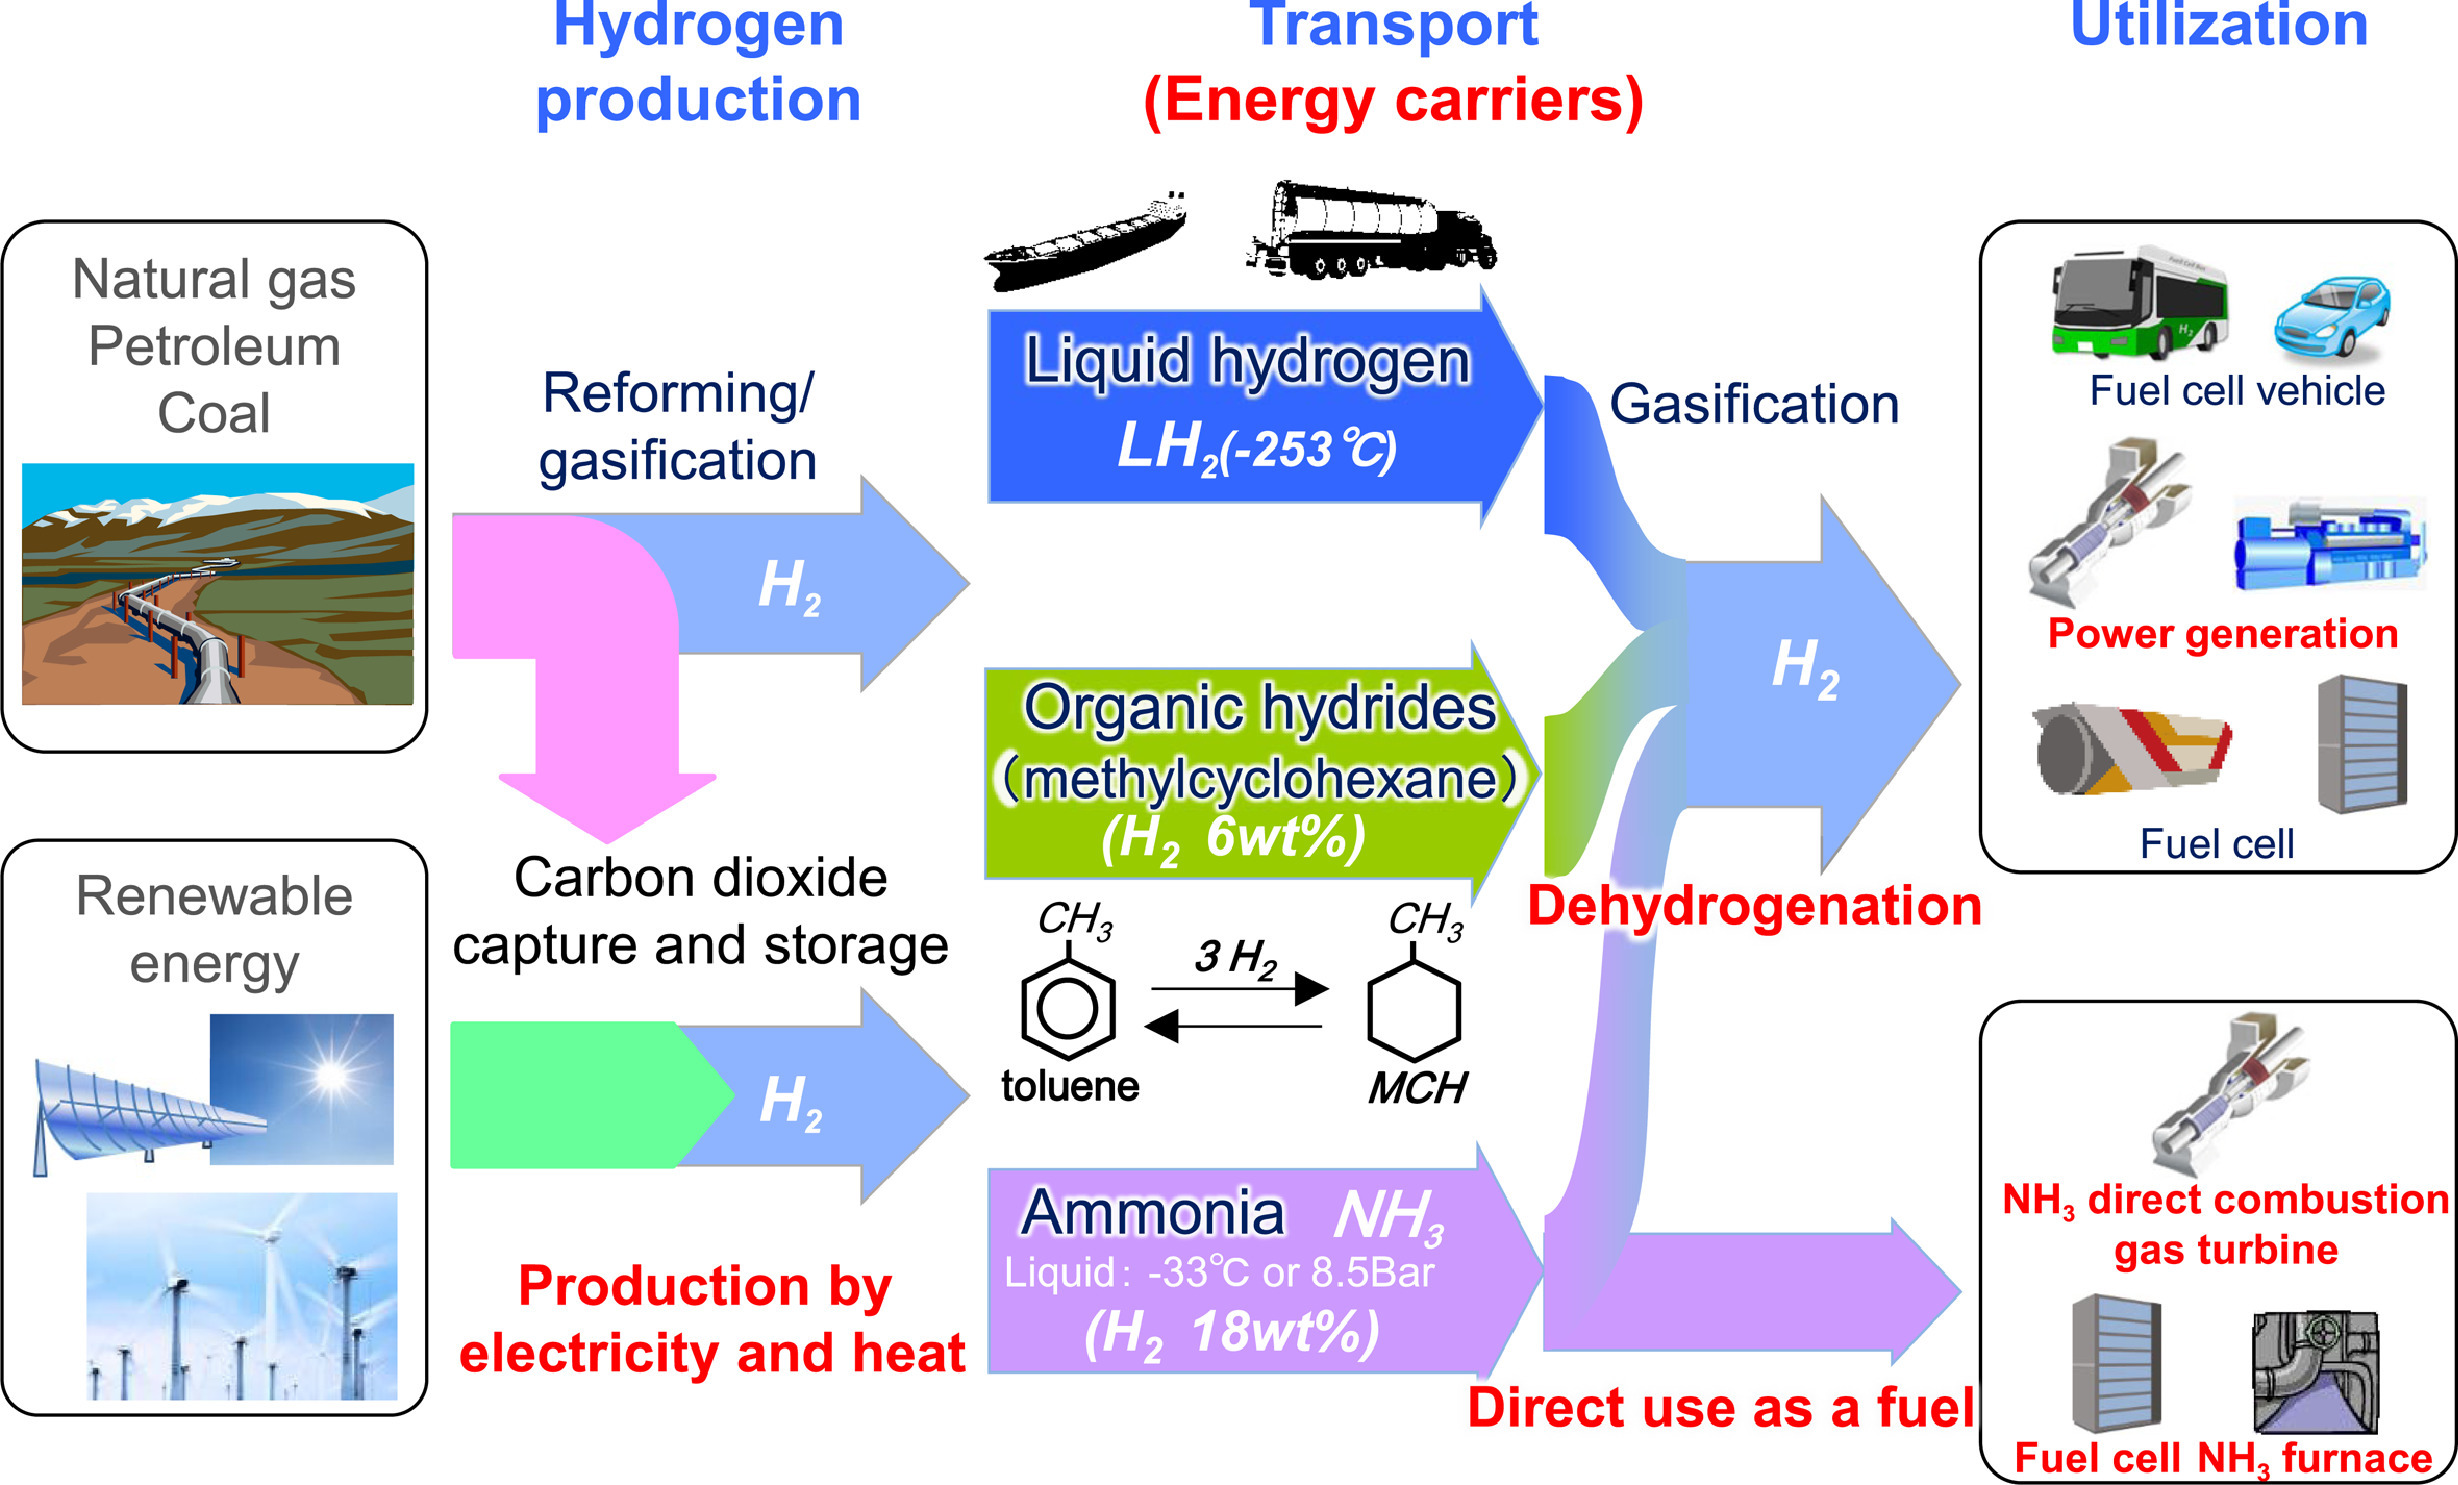
\includegraphics[width=\textwidth]{figures/background.jpg}
			\caption{\fullcite{kobayashiScienceTechnologyAmmonia2019}}
			\end{figure}
		\end{column}
	\end{columns}
\end{frame}

\begin{frame}{Objectives}
	\begin{itemize}
		\item Validate Abe Mechanism, at varying combustion conditions, for fuels:
		\begin{itemize}
			\item NH3/H2/Air
			\item CH4/NH3/Air
		\end{itemize}
		\item Flame properties being evaluated:
		\begin{itemize}
			\item Laminar burning velocity
			\item Specie profiles
			\item Intermediate species profiles
		\end{itemize}
	\item Optimize reaction mechanism to fit experimental data for all conditions above satisfactorily
	\end{itemize}
\end{frame}

\begin{frame}{Prior Findings}
    \setbeamercovered{transparent} 
    
    \begin{itemize}
        \item Validate Abe Mechanism, at varying combustion conditions, for fuels:
        \begin{itemize}
            \item NH3/H2/Air
            \item CH4/NH3/Air
        \end{itemize}
        
        \item Flame properties evaluated:
        \begin{itemize}
            \item Laminar burning velocity
        \end{itemize}
    \end{itemize}
\end{frame}

\begin{frame}{Prior Findings --- NH3/H2/Air}
	Abe mechanism reproduces LBV of NH/H2/Air flame to match experimental data
	\begin{figure}
		\centering
		
\includegraphics[height=0.6\textheight]{figures/lbv_p-1_phi-10.png}
		\caption{Laminar burning velocities of NH3/H2/Air flames at varying H2 concentrations while pressure and equivalence ratio is kept constant at 1atm and 1.0 respectively}
	\end{figure}
\end{frame}

\begin{frame}{Prior Findings --- CH4/NH3/Air}
	Plotting of experimental data from Okafor 2019\footfullcite{okaforMeasurementModellingLaminar2019a} was corrected
	\begin{figure}
		
\includegraphics[height=0.6\textheight]{figures/lbv_p-1_phi-7.png}
		\caption{Laminar burning velocities of CH4/NH3/Air flames at varying NH3 concentrations while pressure and equivalence ratio is kept constant at 1atm and 0.7 respectively}
	\end{figure}
\end{frame}

\begin{frame}{Prior Findings --- Failed Conditions}
	\begin{itemize}
		\item LBV overprediction by Abe mech observed across most CH4/NH3/Air conditions.
		\begin{itemize}
			\item Pressure = 1 atm, $\phi=1.4$
			\item Pressure = 1 atm, $\phi=1.6$
		\end{itemize}
		\item Experimental data for higher pressures, 3atm and 5atm, are lacking for both fuels
		\item Numerical simulations with Okafor reduced mechanism failed to converge
		\begin{itemize}
			\item Unable to compare LBV from Okafor Reduced Mechanism and Abe mech at the conditions discussed
		\end{itemize}
	\end{itemize}
\end{frame}

\begin{frame}{Next Steps}
	\begin{itemize}
		\item Validating Abe mech's specie profiles with experimental data from literature
		\item Speciation data for relevant fuels and corresponding fuels selected
		\begin{itemize}
			\item CH4/NH3: NH3, NO, CO
			\item NH3: OH, NH, NO
			\item NH3/H2: NH2, NH, NOx
		\end{itemize}
		\item For each speciation dataset, simulation methodology employed in the corresponding paper must be used for validating Abe mech
	\end{itemize}
\end{frame}

\begin{frame}{Specie Profiles --- CH4/NH3}
	\begin{itemize}
		\item From \cite{mendiaraAmmoniaChemistryOxyfuel2009}, the speciation data is used to validate NH3, NO and CO profiles
		\item Plug Flow Reactor
		\begin{itemize}
			\item Diameter = 12 mm
			\item Length = 120 cm
			\item Gas flow rate = 1 dm$^3$/min
			\item Temperature = 973-1773 K
		\end{itemize}
	\end{itemize}
	\begin{table}
		\caption{Experimental conditions that need to be simulated with the plug flow reactor. \fullcite{mendiaraAmmoniaChemistryOxyfuel2009}}\label{tab:}
		\centering
		\small
		\setlength{\tabcolsep}{3pt}
		\begin{tabularx}{\textwidth}{@{} l *{6}{C} @{}}
			\toprule
			Run & {$\text{CH}_4/\text{ppm}$} & {$\text{O}_2/\text{ppm}$} & {$\text{NH}_3/\text{ppm}$} & {$\text{N}_2/\%$} & {$\phi$} & Residence time/s \\
			\midrule
			1   & 2515 & 3479  & 484 & 99.35 & 1.55 & $1296/T$ (K) \\
			2   & 2513 & 5036  & 468 & 99.20 & 1.07 & $1296/T$ (K) \\
			3   & 2508 & 40062 & 468 & 95.69 & 0.13 & $1293/T$ (K) \\
			\bottomrule
		\end{tabularx}
	\end{table}
\end{frame}

\begin{frame}{Specie Profiles --- NH3}
	\begin{itemize}
		\item From \cite{brackmannStructurePremixedAmmonia2016a}, speciation data of OH, NH and NO profiles are used to validate Abe mech.
		\item Stagnation Flame Reactor
		\begin{itemize}
			\item Steel disk to stabilize the flame
			\item Flame stabilized at $\sim$6 mm above burner surface so domain should be $>$ 6 mm
			\item Temperature profiles from the experiment used as input
			\item GRAD parameter was set to 0.02
		\end{itemize}
	\end{itemize}
	\begin{table}
		\caption{Experimental conditions that need to be simulated with the stagnation flame reactor. \fullcite{brackmannStructurePremixedAmmonia2016a}}
		\centering
		\small
		\setlength{\tabcolsep}{3pt}
		\begin{tabularx}{\textwidth}{@{} l *{6}{C} @{}}
		\toprule
        Flame & {$\text{NH}_3$} & {Air} & {$\text{N}_2\text{-flame}$} & {$\text{N}_2\text{-coflow}$} \\
              & {($L_{\text{n}}/\text{min}$)} & {($L_{\text{n}}/\text{min}$)} & {($L_{\text{n}}/\text{min}$)} & {($L_{\text{n}}/\text{min}$)} \\
        \midrule
        $\phi = 0.9$ & 2.62 & 10.3 & 0    & 1.2 \\
        $\phi = 1.0$ & 3.38 & 12.1 & 0.87 & 1.2 \\
        $\phi = 1.2$ & 3.9  & 11.6 & 0    & 1.2 \\
        \bottomrule
		\end{tabularx}
	\end{table}
\end{frame}

\begin{frame}{Specie Profiles --- NH3/H2}
	\begin{itemize}
		\item From \cite{alturaifiShocktubeStudyNH32023}, speciation data of NH3, NO, NOx, N2O and NH2 profiles used.
		\item Premixed Laminar Flame-Speed Reactor/Burner-stabilized flat flame
		\begin{itemize}
			\item Domain/width of $\sim20$ mm
			\item Experimental flame's temperature profile used as input
		\end{itemize}
	\end{itemize}
	\begin{table}
		\caption{Experimental conditions that need to be simulated. \fullcite{alturaifiShocktubeStudyNH32023}}
		\centering
		\small
		\setlength{\tabcolsep}{3pt}
		\begin{tabularx}{\textwidth}{@{} l *{7}{C} @{}}
		\toprule
		Flame & \text{$X_{NH_3}$} & \text{$X_{H_2}$} & \text{$X_{O_2}$} & \text{$X_{Ar}$} & \text{$V_0$ (cm/s)} & \text{$\Phi$} & \text{$p$ (mbar)} \\ 
		\midrule
		I    & 0.25 & 0.05 & 0.21 & 0.48 & 35.1 & 1   & 60  \\
		II   & 0.24 & 0.07 & 0.21 & 0.47 & 42.1 & 1   & 50  \\
		III  & 0.22 & 0.10 & 0.21 & 0.46 & 42.1 & 1   & 50  \\
		IV   & 0.21 & 0.13 & 0.21 & 0.45 & 42.0 & 1   & 50  \\
		V    & 0.22 & 0.10 & 0.24 & 0.43 & 42.2 & 0.9 & 50  \\
		VI   & 0.22 & 0.10 & 0.20 & 0.48 & 42.5 & 1.1 & 50  \\
		VII  & 0.25 & 0.05 & 0.21 & 0.48 & 23.4 & 1   & 90  \\
		VIII & 0.25 & 0.05 & 0.21 & 0.48 & 17.6 & 1   & 120 \\
		\bottomrule
		\end{tabularx}
	\end{table}
\end{frame}

\begin{frame}[plain] % plain removes headers/footers
    \centering
	\setbeamercolor{textbf}{bg=kyushu}
	\Huge \textbf{Thank You}
\end{frame}   

\end{document}
